\documentclass{article}
\usepackage[utf8]{inputenc}
% \usepackage[margin=1.75in]{geometry}
\usepackage[left=1.5in,right=1.5in,top=1in,bottom=1in]{geometry}
\usepackage{graphicx}
\usepackage{hyperref}
\usepackage{xcolor}
\usepackage{fontawesome}
\usepackage[nottoc]{tocbibind} %Includes "References" in the table of contents
\usepackage{listings}
\usepackage{textcomp}

\definecolor{mGreen}{rgb}{0,0.6,0}
\definecolor{mGray}{rgb}{0.5,0.5,0.5}
\definecolor{mPurple}{rgb}{0.58,0,0.82}
% \definecolor{backgroundColour}{rgb}{0.95,0.95,0.92}
\definecolor{backgroundColour}{HTML}{F2F2F2}

\lstdefinestyle{CStyle}{
    backgroundcolor=\color{backgroundColour},
    commentstyle=\color{mGreen},
    keywordstyle=\color{magenta},
    numberstyle=\tiny\color{mGray},
    stringstyle=\color{mPurple},
    basicstyle=\footnotesize,
    breakatwhitespace=false,         
    breaklines=true,                 
    captionpos=b,                    
    keepspaces=true,                 
    numbers=left,                    
    numbersep=5pt,                  
    showspaces=false,
    showstringspaces=false,
    showtabs=false,                  
    tabsize=2,
    language=C,
    basicstyle=\ttfamily\scriptsize,
    frame=single,
    % xleftmargin=3.4pt,
    % xrightmargin=3.4pt,
}

\definecolor{link}{HTML}{0066cc}

\hypersetup{
    colorlinks=true,
    linkcolor=link,
    filecolor=magenta,      
    urlcolor=link,
    citecolor=link
}

\graphicspath{ {images/} }

\title{Cache and Multi-Core Efficient Algorithms for High-Degree Permutations}
\author{
    Steve Linton and Ryan Gibb\\
    University of St Andrews\\
    \{sl4, rtg2\}@st-andrews.ac.uk\\
    }
\date{October 2020}

\begin{document}

\maketitle

\section*{Abstract}

% The area of the paper (1 sentence). The problem area to which this paper makes a contribution.
% The issue the paper addresses (1 sentence). Presumably the area is not yet fully explored, and you've found a problem that needs tackling otherwise what's in your paper?
% What you've done, the results you've obtained (2 sentences). The key contribution of the paper, what you've added to practice and/or knowledge
% What this means (1 sentence). Why should anyone care?

The traditional naive permutation composition algorithm is limited by memory latency and not CPU speed. Algorithms to take advantage of current memory hierarchies and multiple cores can be designed so as to be limited by memory bandwidth instead. We have implemented and benchmarked a number of such algorithms. We have found a multithreaded Rust implementation of the naive algorithm is 64\% than the naive algorithm on an Intel Xeon E3-1230 v5 with 64GB RAM for permutations of degree $2^{32}$. This can be adapted to improve the performance of other permutation operations, as well as other algorithms that access large amounts of main memory pseudo-randomly.



\section{Introduction}

%CPU-memory gap
%Memory wall

Work was done on creating a permutation composition algorithm to overcome this `memory wall' in 2002 by Cooperman and Ma using a bucket algorithm to make effect use of the cache.\cite{Cooperman2002OvercomingTM} This algorithm will be refer to as the `Cooperman \& Ma algorithm' hereafter. We will see how their algorithm holds up on modern hardware for significantly larger permutations  - up to $n=2^{32}$ compared to the previous $n=2^{20}$.

The other algorithms considered are the naive algorithm as a baseline, a multithreaded naive algorithm, a multithreaded Cooperman \& Ma algorithm, and a vector optimised naive algorithm.



\section{Design}

A permutation $\sigma$ of degree $n$ is a bijective function from a set $S=\{1, \ldots, n\}$ onto itself, represented as an array $x$ of length $n$ where the value at index $i$ in the array is the image of $i$ under $\sigma$. More simply, if $\sigma(i)=j$ then \texttt{x[i]=j}.

Given two permutations $i\mapsto \sigma(i)$ and $i\mapsto \pi(i)$, their composition $\sigma\pi$ is defined as $i\mapsto \pi(\sigma(i))$.

Taking two permutations \texttt{x} and \texttt{y}, the following algorithms calculate their composition \texttt{z=xy}. All of \texttt{x}, \texttt{y}, and \texttt{z} must of length \texttt{n}, with \texttt{x} and \texttt{y} containing every value from \texttt{0} to \texttt{n - 1} exactly once.

Let \verb|perm_t| be the type of the permutation arrays; the type of the elements in the permutation image. This determines the maximum permutation degree than can be composed; as well as the number of bytes used to store the permutation \texttt{n*sizeof(perm\_t)}.

% TODO give pseudocode

\subsection{Naive}

\begin{lstlisting}[style=CStyle, caption={Naive Algorithm}]
perm_t x[n], y[n], z[z];

for (size_t i = 0; i < n; i++) {
	z[i] = y[x[i]];
}
\end{lstlisting}

% \clearpage
\subsection{Cooperman \& Ma}

Note \texttt{CACHE\_SIZE} is the number of bytes in the target cache.

\begin{lstlisting}[style=CStyle, caption={Cooperman \& Ma Algorithm\cite{Cooperman2002OvercomingTM}}]
#define BLOCK_LENGTH (CACHE_SIZE / 2 / sizeof(int))
#define NUMBER_OF_BLOCKS = (n / BLOCK_LENGTH)

perm_t x[n], y[n], z[z];
perm_t d[n];
perm_t* d_ptr[NUMBER_OF_BLOCKS];

//Phase I: distribute value, x[a], into d_ptr[block_num]
// such that block_num == x[a] / BLOCK_LENGTH
for (size_t block_num = 0; block_num < NUMBER_OF_BLOCKS; block_num++) {
    d_ptr[block_num] = &d[block_num * BLOCK_LENGTH];
}
for (size_t i = 0; i < ARRAY_LENGTH; i++) {
    block_num = x[i] / BLOCK_LENGTH;
    *d_ptr[block_num] = x[i];
    d_ptr[block_num]++;
}

//Phase II: for d[i] == x[a], replace the value x[a] by y[x[a]]
// Note that |i - d[i]| == |i - x[a]| and |i-x[a]| < BLOCK_LENGTH
for (size_t i = 0; i < ARRAY_LENGTH; i++) {
    d[i] = y[d[i]];
}

//Phase III: copy value y[x[a]] from d_ptr[block_num] to \[a]
for (size_t block_num = 0; block_num < NUMBER_OF_BLOCKS; block_num++) {
    d_ptr[block_num] = &d[block_num * BLOCK_LENGTH];
}
for (int i = 0; i < ARRAY_LENGTH; i++) {
    block_num = x[i] / BLOCK_LENGTH;
    z[i] = * d_ptr[block_num];
    d_ptr[block_num]++;
}

\end{lstlisting}

\subsection{Multithreaded Naive}

% Assume the existence of a function \texttt{SPAWN\_THREAD} that spawns a thread to execute the given function with the given list of parameters, and a function \texttt{JOIN\_THREADS} which waits for all the spawned threads to finish execution.

% \begin{lstlisting}[style=CStyle]
% void composition_multithread_naive_thread(size_t n, int x[], int y[], int z[]) {
%     for (int i = 0; i < slice_length; i++) {
%         z[i] = y[x[i]]
%     }
% }

% // Ensure each thread operates on a cache line boundary.
% int elements_per_cache_line = CACHE_LINE_BYTES / sizeof(int);
% double elements_per_thread = (double) n / THREADS;
% // If there are less elements per thread than fit in a cache line,
% if (elements_per_thread < (double) elements_per_cache_line) {
%     // Create a thread for each cache line's worth of elements.
%     THREADS = n / elements_per_cache_line;
%     elements_per_thread = (double) n / THREADS;
% }
% double cache_lines_per_thread
%     = elements_per_thread / elements_per_cache_line;

% if (THREADS > 1) {
%     // Assign each thread to a different chunk of x and z.
%     int x_tail[] = x;
%     int z_tail[] = z;
%     int index = 0;
%     for (int thread_id = 0; thread_id < THREADS; thread_id++) {
%         size_t l = (size_t) thread_id * cache_lines_per_thread;
%         size_t h = (size_t) (thread_id + 1) * cache_lines_per_thread;
%         let length = (h - l) * elements_per_cache_line;
%         index += length;
%         SPAWN_THREAD(
%             composition_multithread_naive_thread, length, x_tail, y, z_tail
%         );
%         x_tail = &x_tail[length];
%         z_tail = &z_tail[length];
%     }
%     composition_multithread_naive_thread(n - index, x_tail, y, z_tail);
% } else {
%     composition_multithread_naive_thread(n, x, y, z);
% }
% JOIN_THREADS()
% \end{lstlisting}

This algorithm splits the permutation into different slices of \texttt{x} and \texttt{z}, and runs a thread for each slice to naively compose them in parallel. The number of threads should not exceed the number of CPU cores. Note \texttt{y} is shared between all threads.

\subsection{Multithreaded Cooperman \& Ma}

Phase 2 of the algorithm is run in parallel with the `blocks' in \texttt{d} distributed between threads and each thread operating on a number of blocks independently. As with multithreaded naive the number of threads should not exceed the number of CPU cores and \texttt{y} is shared between all threads.

\subsection{Naive Optimised}

Signed \verb|perm_t| values, the restrict type qualifier for permutation array arguments to the function, and compilation with the \texttt{-march=native} flag (to target the compilation machine's hardware), results in assembly code using vector optimisations.

% \subsection{Unrolled}

% This algorithm `unrolls' the naive implementation loops to not rely on out of order execution. A number of elements (\texttt{ROLLS}) are read from x and stored in an array, then the same number. The idea is to cut down on the time waiting on memory latency but requesting the next \texttt{x} value while the previous one is being sent.

% \begin{lstlisting}[style=CStyle]
% #define ROLLS 4

% perm_t x[n], y[n], z[z];

% perm_t rolls[ROLLS];
% size_t n_rounded = (n / ROLLS) * ROLLS;
% for (size_t i = 0; i < n_rounded; i += ROLLS) {
%     // Read ROLLS values from x, and write then to z
% 	for (size_t j = 0; j < ROLLS; j++) {
% 		rolls[j] = x[i + j];
% 	}
% 	// Read ROLLS values from y, and write then to z
% 	for (size_t j = 0; j < ROLLS; j++) {
% 		z[i + j] = y[rolls[j]];
% 	}
% }
% size_t i = n_rounded;
% size_t leftover_n = n - n_rounded;
% for (size_t j = 0; j < leftover_n; j++) {
% 	rolls[j] = x[i + j];
% }
% for (size_t j = 0; j < leftover_n; j++) {
% 	z[i + j] = y[rolls[j]];
% }
% \end{lstlisting}

% Using the appropriate optimisation flags the inner loops (using the \texttt{j} counter) are expanded; that is they the instructions inside them are duplicated \texttt{ROLLS} times with incrementing values of j hardcoded.



\section{Implementation}

The naive and Cooperman \& Ma algorithms were implemented in C and Rust to ensure using Rust wasn't effecting performance. The multithreaded algorithms were written in Rust for efficient memory safety. The naive optimised and unrolled algorithms were implemented in C for fine grained optimisation and compilation control.

The implementations here aren't included for the sake of brevity as they are either essentially the same as the algorithm design or are obfuscated by optimisations.

Timings were done with calls to \texttt{clock\_gettime}. Wall clock time was used, as opposed to CPU time, due to the latter's complications with multithreading. If the composition took less than 10 milliseconds the number of times the composition was done was doubled (growing exponentially) with a loop in between the \texttt{clock\_gettime} calls until it took 10 milliseconds or more. This was done to remove issues with the accuracy of the system call for very small intervals. It's possible this may give faster than actual results for small permutations due to caching, but the effects should be consistent across algorithms.

The repository can be found at \href{https://github.com/RyanGibb/uras-permutations}{github.com/RyanGibb/uras-permutations}, containing the implementations, assembly, testing script, benchmarking script, and benchmark CSV file.
%, and the implementations in Rust at\par \href{https://github.com/RyanGibb/uras-permutations/tree/master/rust/src}{https://github.com/RyanGibb/uras-permutations/tree/master/rust/src}.


\clearpage
\section{Results}

% TODO run benchmarks on quiet system and import graphs

\begin{figure}[h]
    \centerline{
        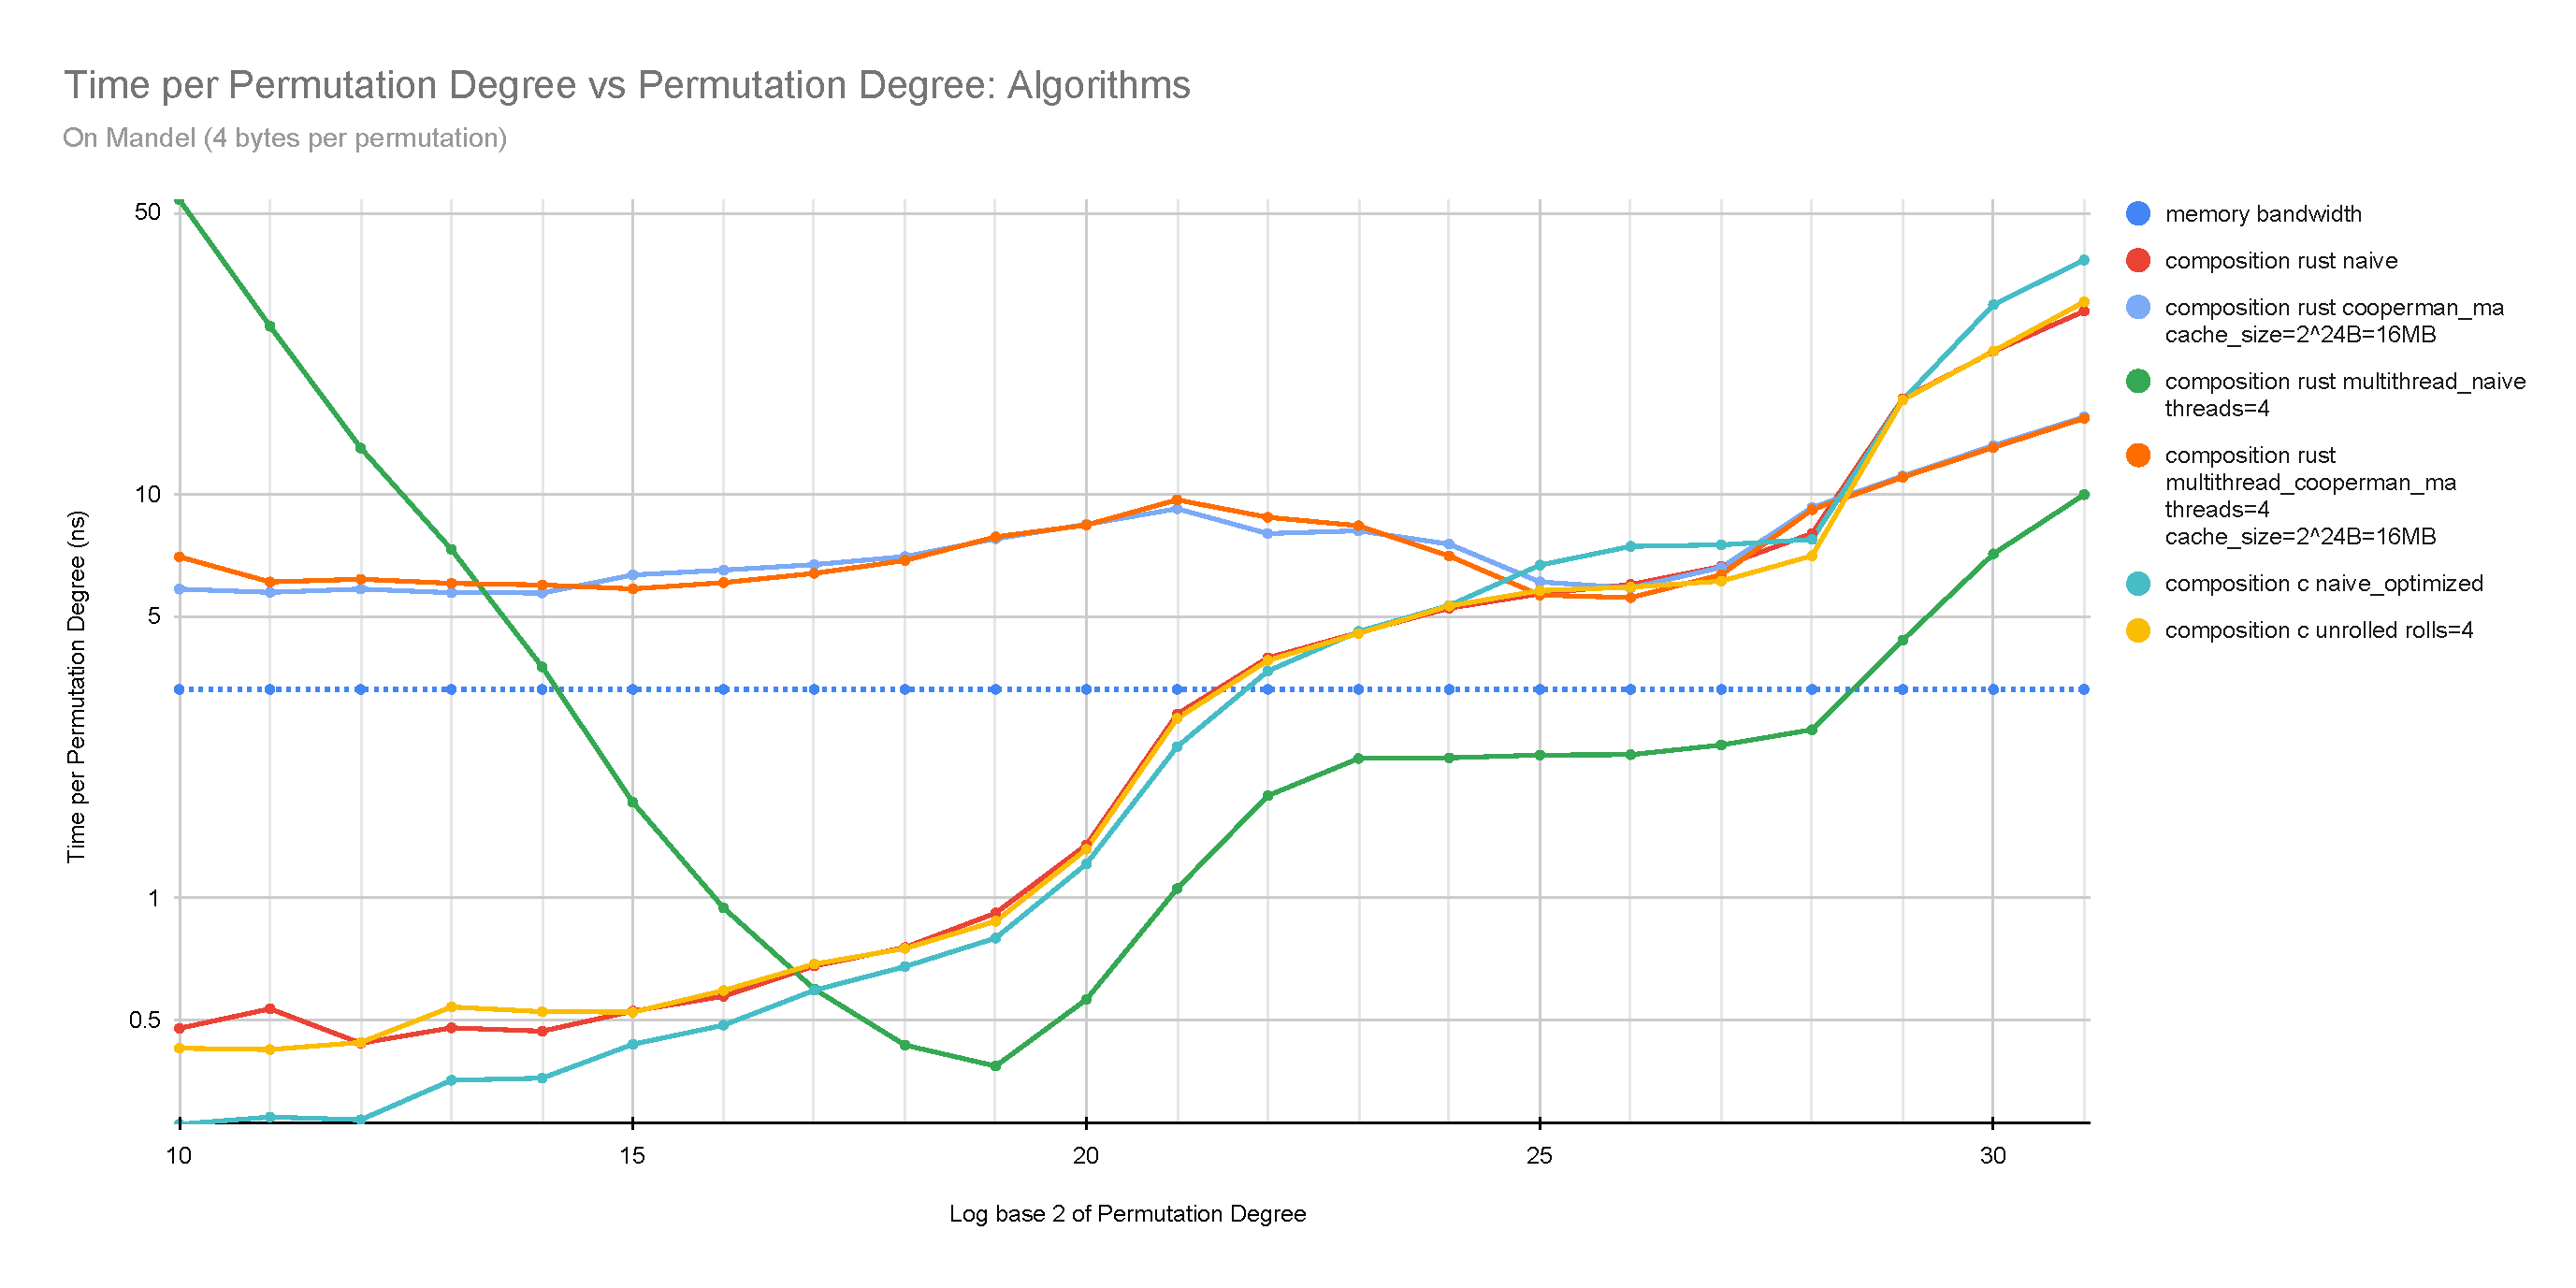
\includegraphics[width=0.9\paperwidth,height=\textheight,keepaspectratio]
        {Time per Permutation Degree vs Permutation Degree_ Algorithms_mandel.pdf}
    }
    \caption{Time per Permutation Degree vs Permutation Degree}
    \label{fig:1}
\end{figure}

`On Mandel' refers the the machine that the benchmarks were done on. It has an Intel Xeon E3-1230 v5 and 64GB RAM. 4 bytes were used per permutation, giving a maximum permutation size of $2^{4*8=}2^{32}$. The amount of memory used per algorithm can be calculated by 3 (for of \verb|x|, \verb|y|, and \verb|z| permutations) times the degree of the permutation times 4 bytes per permutation. For example, the largest included here is for permutations of degree $2^{32}$, so $3*2^{32}*4\approx51GB$.

The blue dotted line shows the memory bandwidth shows as 19.45 bytes per nanosecond for all reads, as measured by Intel\textsuperscript{\tiny\textregistered} Memory Latency Checker v3.9\cite{latency}. This is the theoretical limit of the performance of the algorithms on this hardware as the permutation size approaches infinity.

When the algorithms outperform this it is due to caching. For example in figure \ref{fig:1}, this limit is crossed for permutations of degree $2^{21}$, at $2^{21}*4\approx8MB$ per permutation. This is explained by the CPU having a shared L3 cache size of 8MB\cite{ark}. The reason why this is the size of one permutation, and not three, is because only \verb|y| is being accessed randomly; \verb|x| and \verb|z| and read and written respectively sequentially. 

The exception to this is \verb|rust multithreaded_naive|. We can see the overhead of this is high for small permutations, but outperforms the non-multithreaded algorithms for degrees larger than $2^{18}$ which is about $1MB$. It plateaus from $2^{23}*4=16MB$ to $2^{28}*4=1GB$ where it finally fails to break the barrier.

\begin{figure}[h]
    \centerline{
        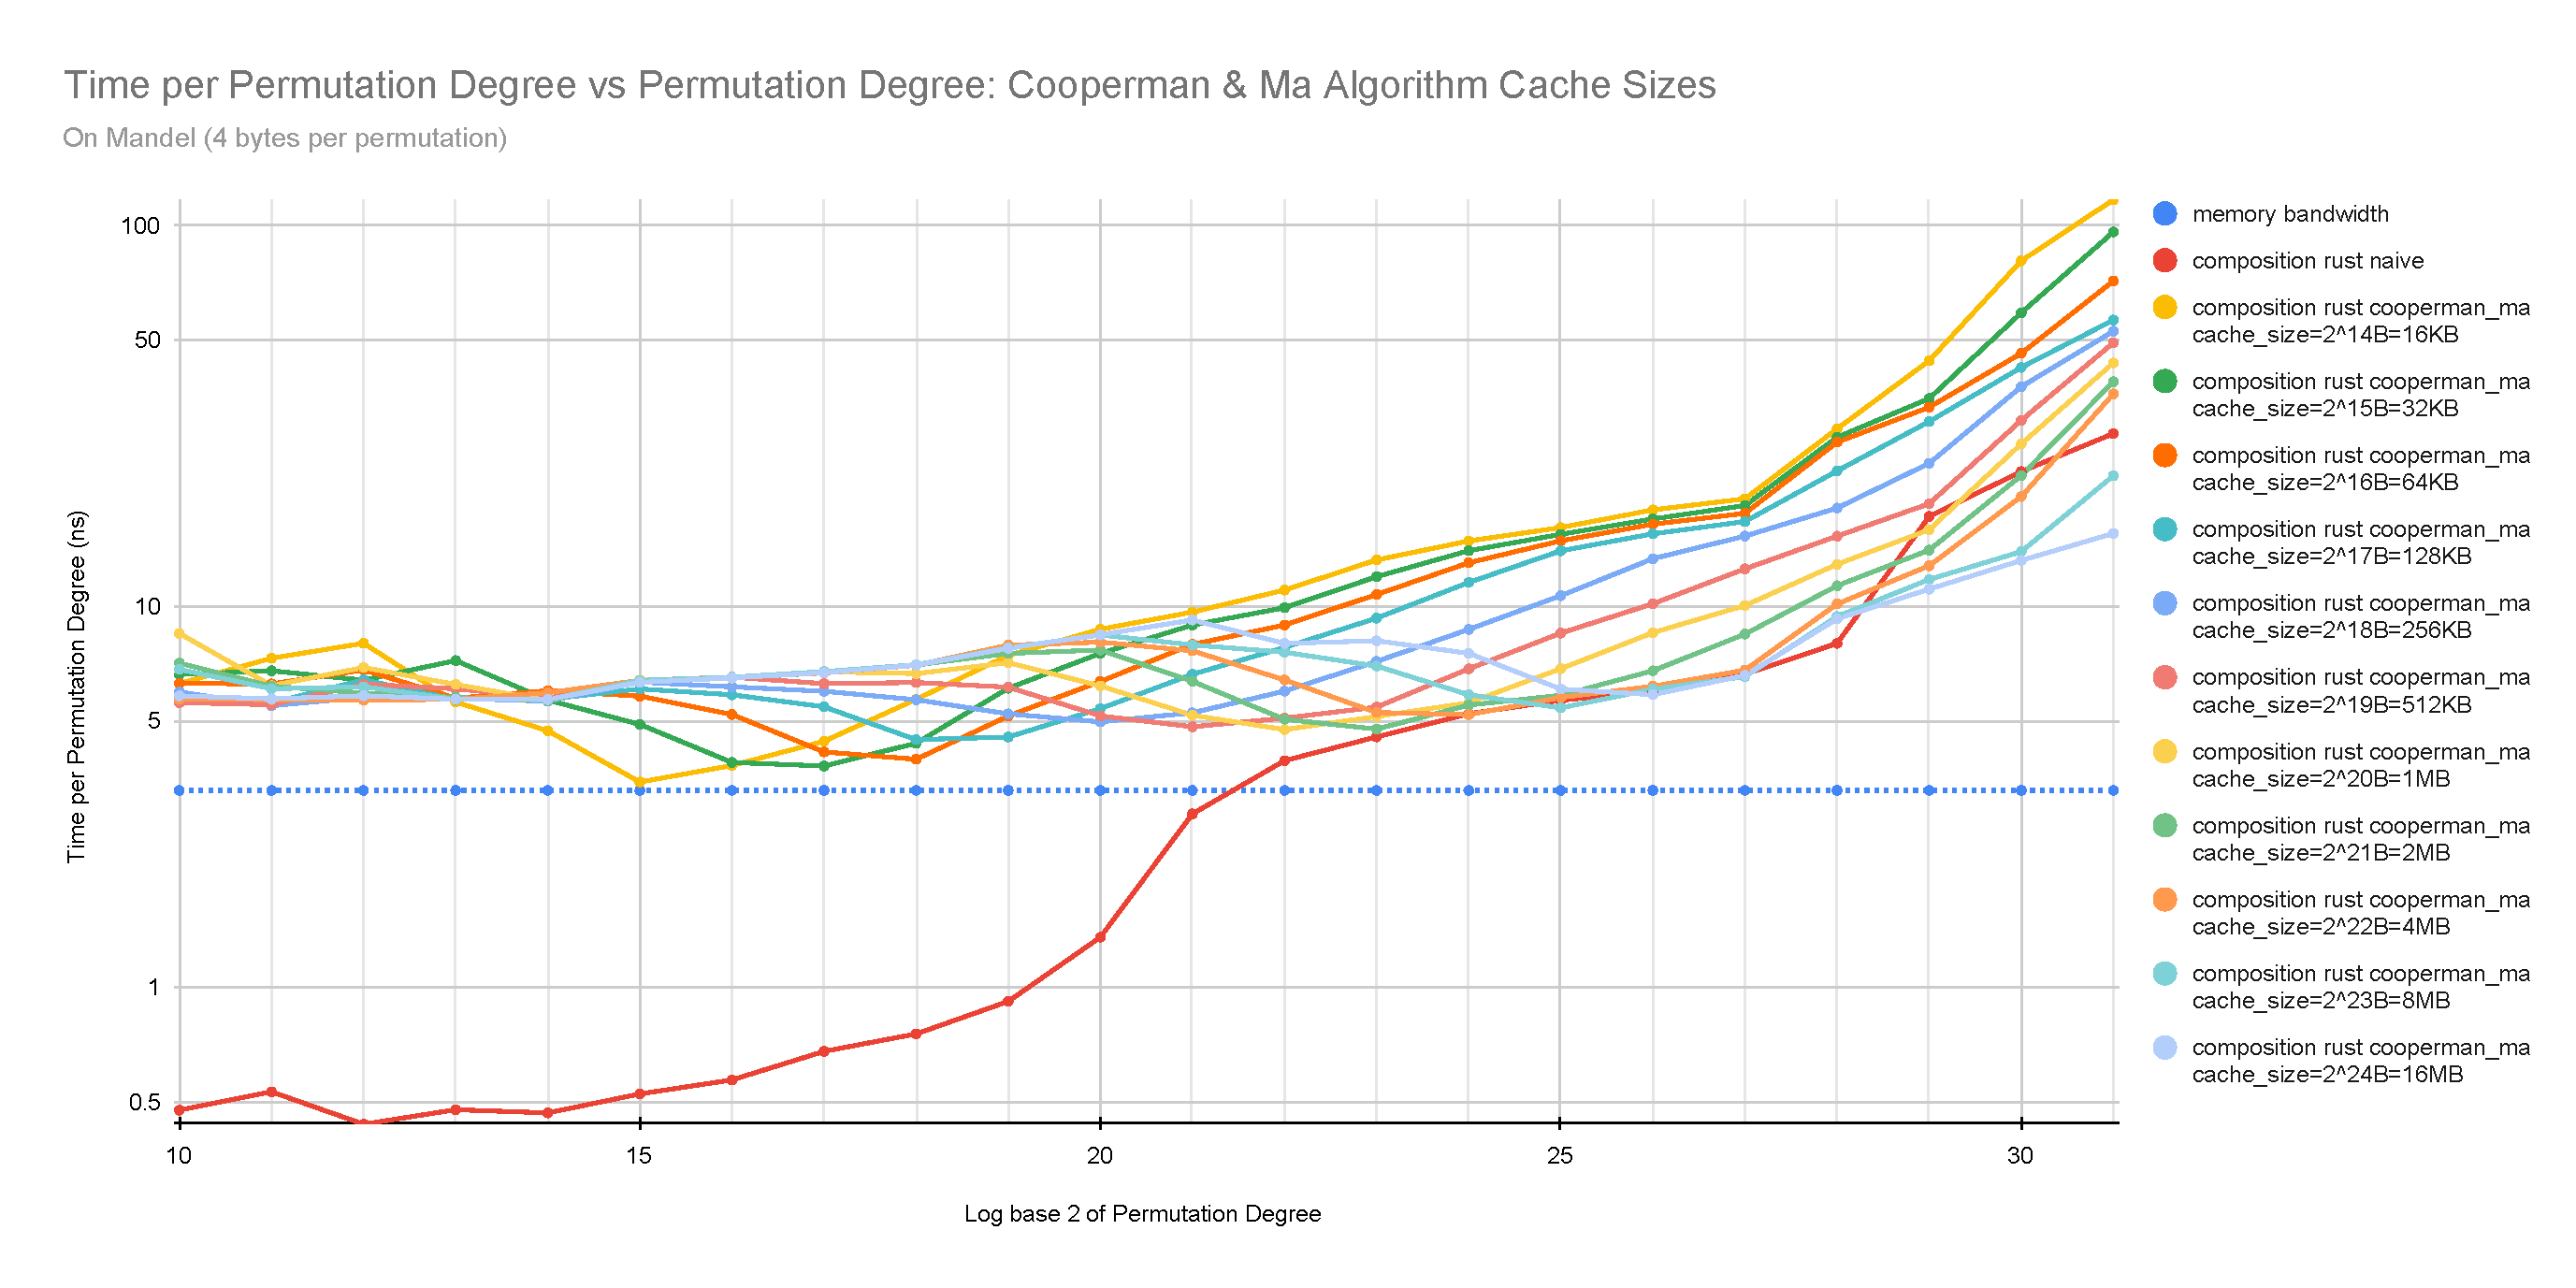
\includegraphics[width=0.9\paperwidth,height=\textheight,keepaspectratio]
        {Time per Permutation Degree vs Permutation Degree_ Cooperman & Ma Algorithm Cache Sizes_mandel.pdf}
    }
    \caption{Cooperman \& Ma Algorithm Cache Sizes}
    \caption{ C}
    \label{fig:2}
\end{figure}

\begin{figure}[h]
    \centerline{
        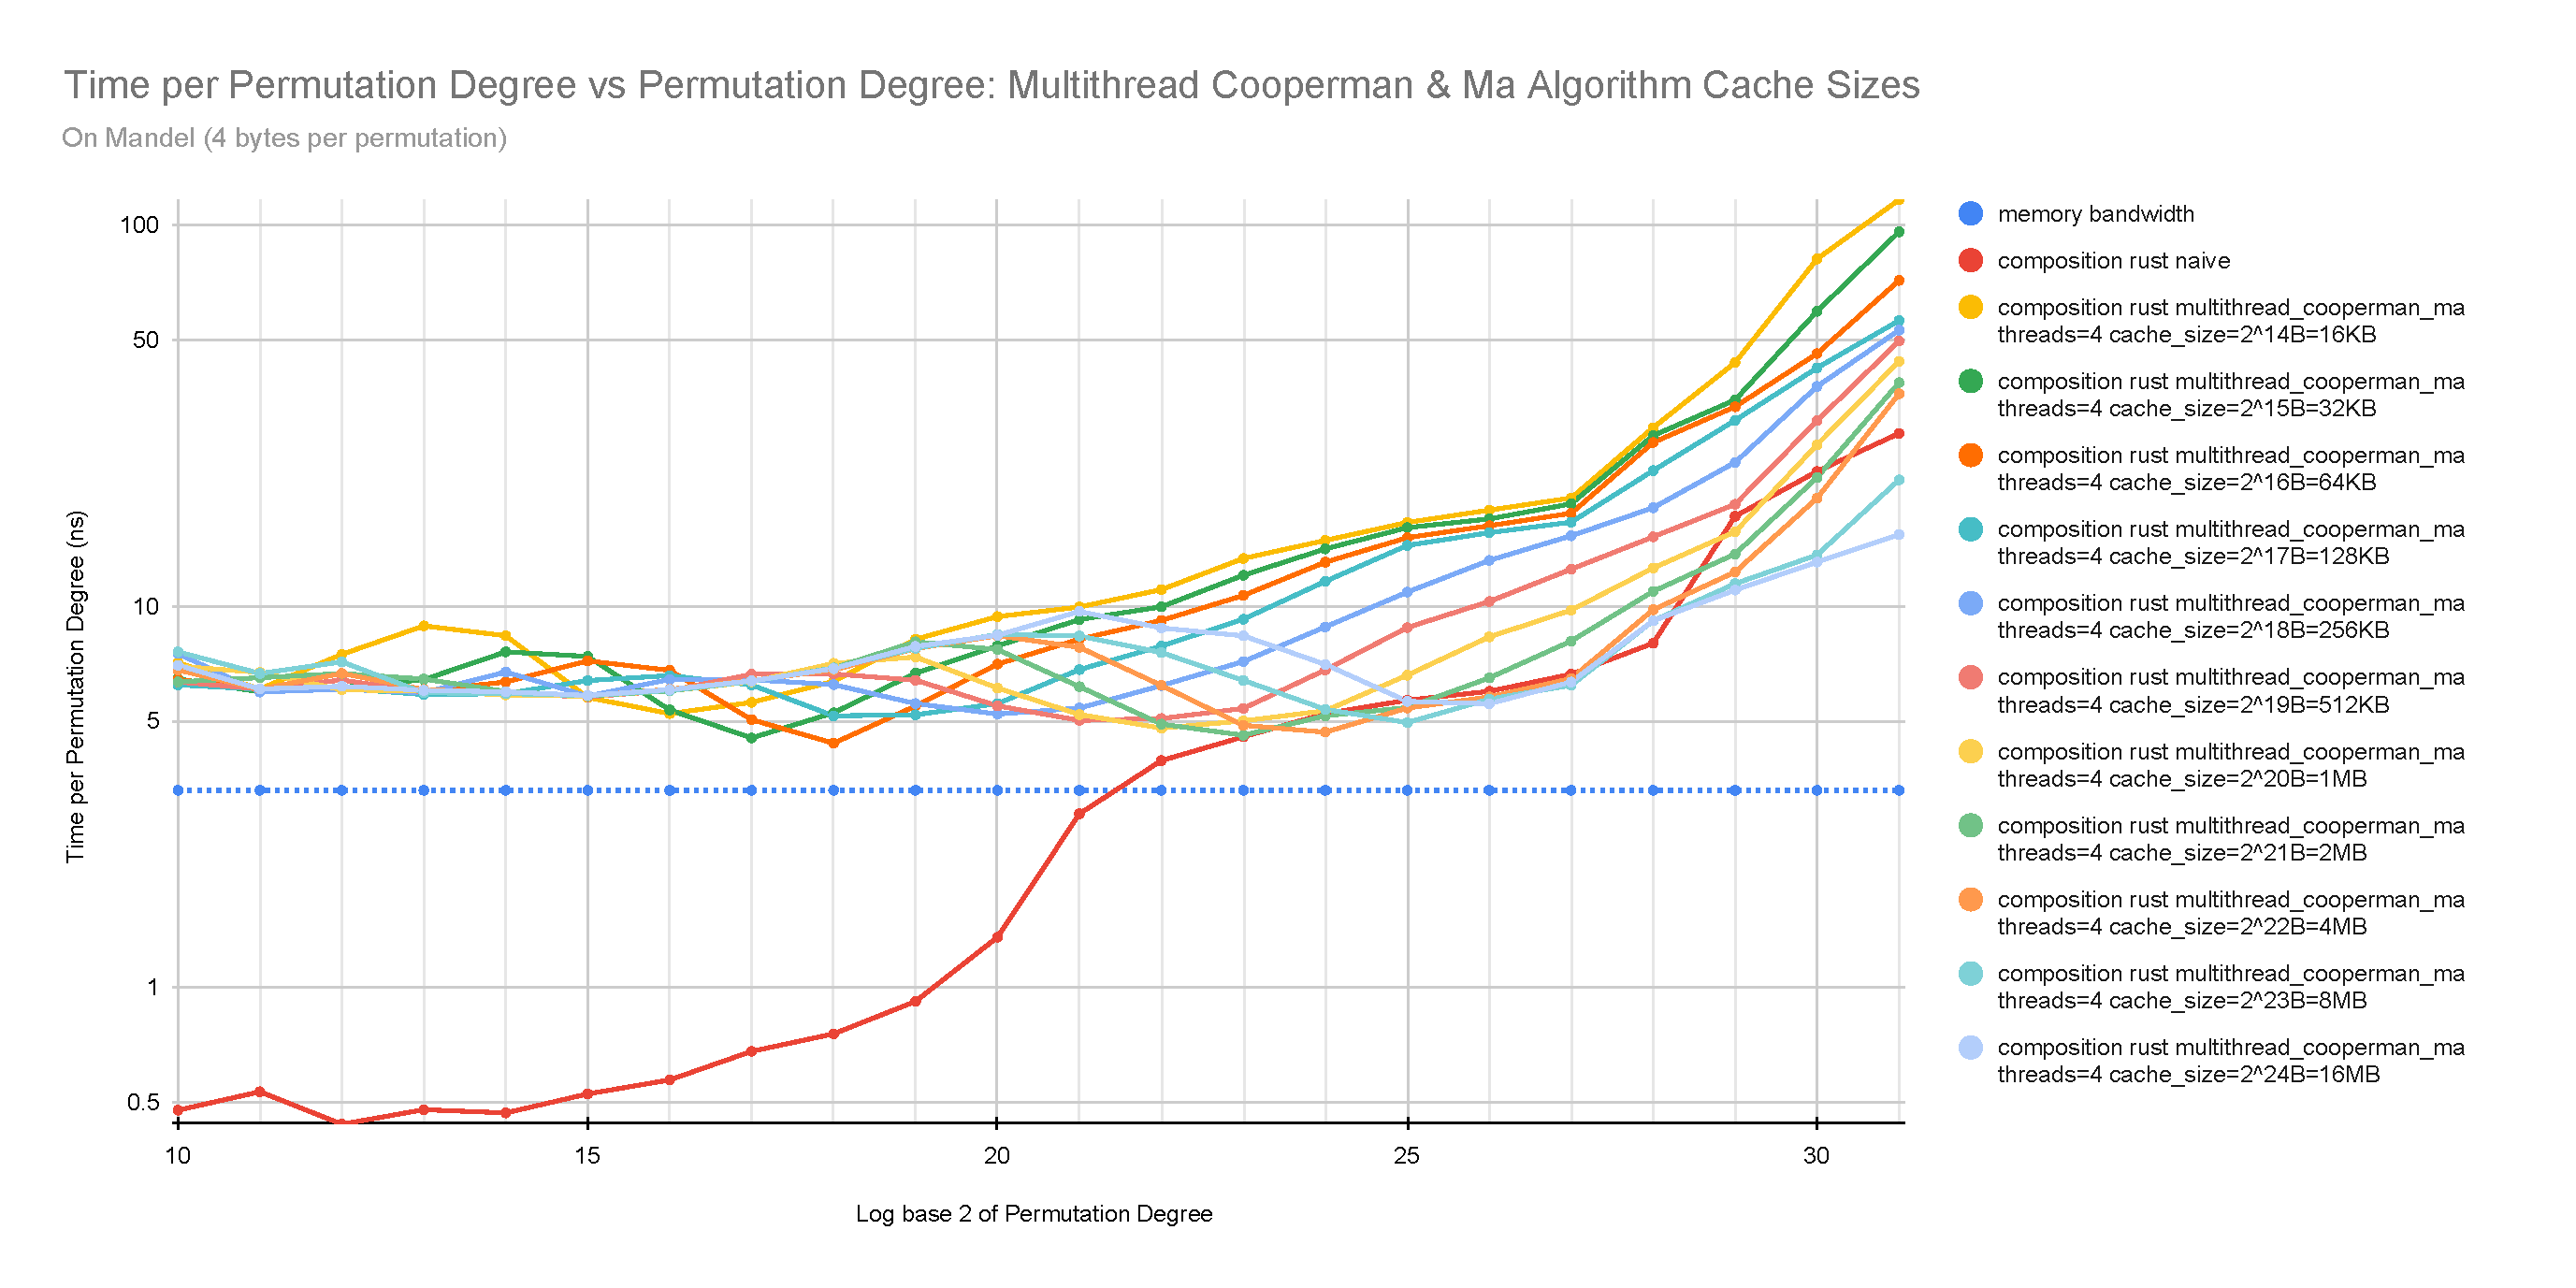
\includegraphics[width=0.9\paperwidth,height=\textheight,keepaspectratio]
        {Time per Permutation Degree vs Permutation Degree_ Multithread Cooperman & Ma Algorithm Cache Sizes_mandel.pdf}
    }
    \caption{Multithread Cooperman \& Ma Algorithm Cache Sizes}
    \label{fig:3}
\end{figure}

\clearpage

Figures \ref{fig:2} and \ref{fig:3} were used to determine the optimal cache size for single threaded and multithreaded Cooperman \& Ma algorithms respectively.
The naive algorithm was included as a comparison.

% Unrolled - This suggests the out of order execution of the naive algorithm works well.


% TODO Analysis of graphs
% Talk about Cooperman & Ma cache sizes
% TODO talk about NUMA?



\section{Conclusion}

% TODO

As can be seen the multithreaded naive algorithms outperform the bucket Copperman \& Ma algorithm.
Further work to be done includes exploring the effects of a multi-level bucket algorithm to take advantage of L1 and L2 caches and different memory latency's in NUMA systems; and creating an optimised multi-core bucket algorithm, building on the multithreaded Cooperman \& Ma algorithm.
%(although the majority of the speed up should come from the L3 cache)

More investigation into the multithreaded algorithm outperforming the bandwidth limit for permutations up to $2^28$ is required. It is possibly a result of the non-NUMA architecture.
It is also possible that the latency results are simply slightly pessimistic.

Investigation into dynamically choosing the algorithm for different hardware and permutation sizes is another avenue of interest.

\bibliographystyle{unsrt}
\bibliography{bibliography}

\end{document}
